\documentclass[tikz, convert]{standalone}

\begin{document}
    
    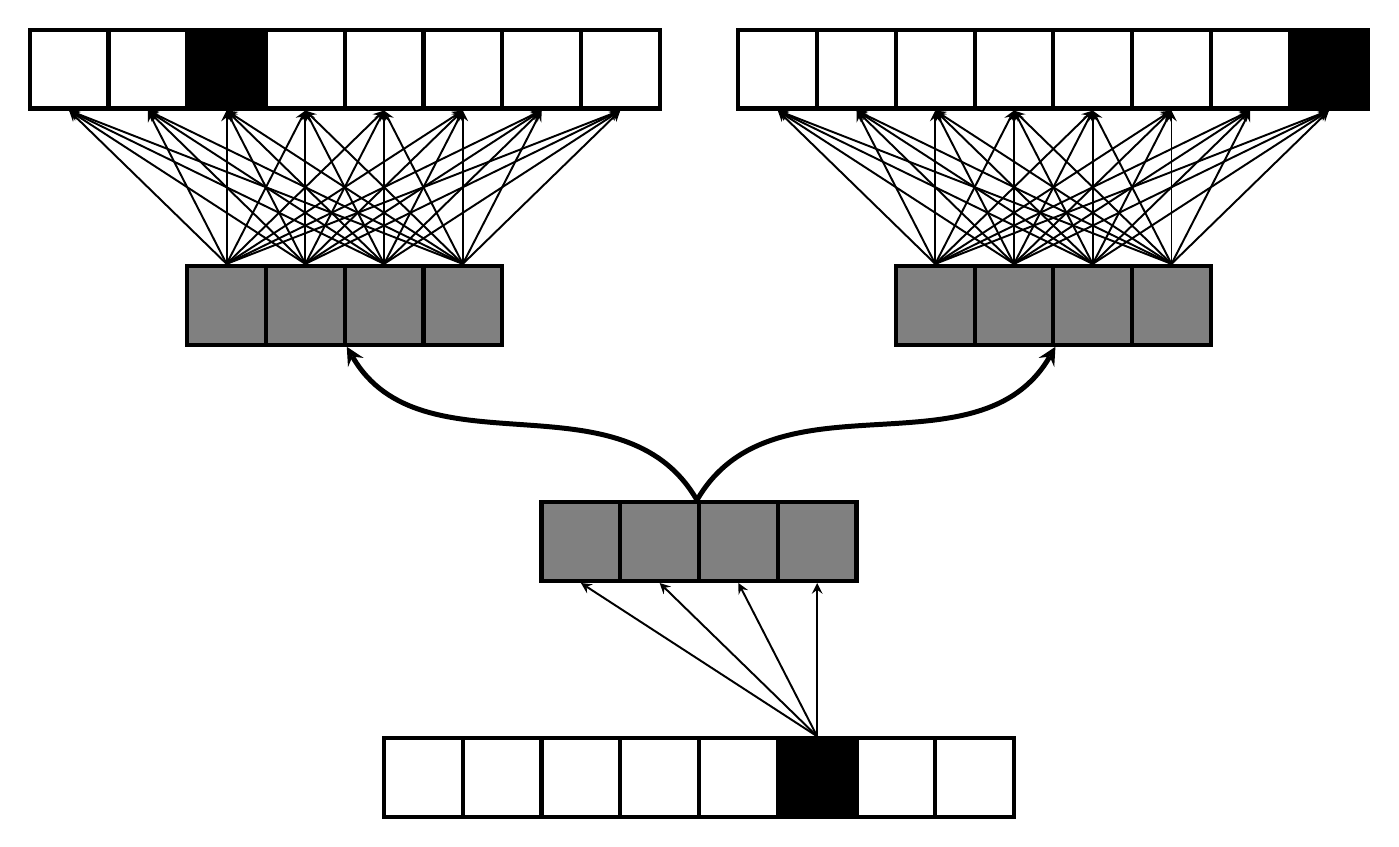
\begin{tikzpicture}[->, >=stealth, every node/.style={rectangle, line width=1.5pt, draw, minimum width=1cm, minimum height=1cm, font=\bfseries}]
    \label{CBOW}
        
        % Input.
        \foreach \x in {-4,...,3}
            \node[xshift=0.5cm] (I-\x) at (\x,0) {};
        \node[fill=black, xshift=0.5cm] (I-1) at (1,0) {};
        
        % Embedding.
        \foreach \x in {-2,...,1}
            \node[xshift=0.5cm, fill=gray] (E-\x) at (\x,3) {};
        % Embedding connections.
        \foreach \dest in {-2,...,1}
            \path[line width=0.7pt] (I-1.north) edge (E-\dest.south);
        
        % Split embedding.
        \foreach \x in {-6,...,-3}
            \node[fill=gray] (E_1-\x) at (\x,6) {};
        \foreach \x in {3,...,6}
            \node[fill=gray] (E_2-\x) at (\x,6) {};
        
        \path[->, line width=1.8pt] (E-0.north west) edge [out=120, in=300] (E_1--5.south east);
        \path[->, line width=1.8pt] (E-0.north west) edge [out=60, in=240] (E_2-4.south east);
        
         % First Output.
        \foreach \x in {-8,...,-1}
            \node (O_1-\x) at (\x,9) {};
        \node[fill=black] (O_1--6) at (-6,9) {};
        
        % Second Output.
        \foreach \x in {1,...,8}
            \node (O_2-\x) at (\x,9) {};
        \node[fill=black] (O_2-8) at (8,9) {};
        
        % Output connections.
        \foreach \source in {-6,...,-3}
            \foreach \dest in {-8,...,-1}
                \path[line width=0.7pt] (E_1-\source.north) edge (O_1-\dest.south);
        \foreach \source in {3,...,6}
            \foreach \dest in {1,...,8}
                \path[line width=0.7pt] (E_2-\source.north) edge (O_2-\dest.south);
        
    \end{tikzpicture}
    
\end{document}